%!TEX program = xelatex
\documentclass[8pt, landscape, a4paper]{extarticle}

% --- 核心宏包 ---
\usepackage[UTF8, fontset=fandol]{ctex}
\usepackage[margin=0.8cm, top=1cm, bottom=1.3cm]{geometry}
\usepackage{multicol}
\usepackage{xcolor}
\usepackage{tcolorbox}
\usepackage{enumitem}
\usepackage{amsmath}
\usepackage{amssymb}
\usepackage{fontspec}
\usepackage{tikz}
\usetikzlibrary{arrows.meta, shapes, decorations.markings}

% --- 去掉页码 ---
\pagestyle{empty}

% --- 颜色定义 (Blue 主题) ---
\definecolor{headerblue}{RGB}{41, 128, 185}    % Belize Hole
\definecolor{navcolor}{RGB}{211, 84, 0}        % 导航橙
\definecolor{intuitioncolor}{RGB}{22, 160, 133}% 直觉绿
\definecolor{accentcolor}{RGB}{192, 57, 43}    % 强调红
\definecolor{section2}{RGB}{142, 68, 173}      % 紫色
\definecolor{dividergray}{RGB}{220, 220, 220}

% --- 全局设置 ---
\setlength{\parindent}{0pt}
\setlength{\columnsep}{0.4cm} 
\linespread{1.1} 

% --- 列表样式 ---
\setlist[itemize]{leftmargin=1.2em, nosep, itemsep=2pt, topsep=2pt, label=$\textcolor{headerblue}{\vcenter{\hbox{\tiny$\bullet$}}}$ }
\setlist[description]{leftmargin=0.2em, style=sameline, nosep, itemsep=2pt, font=\bfseries}

% --- Box 样式 ---
\newtcolorbox{mybox}[2][]{%
  colback=white,
  colframe=#2,
  coltitle=white,
  boxrule=1pt,             
  arc=2mm,                 
  left=4pt, right=4pt, top=3pt, bottom=3pt, 
  toptitle=3pt, bottomtitle=3pt, 
  fonttitle=\bfseries\sffamily\large,
  title={#1},
  after skip=5pt          
}

% --- 自定义命令 ---
\newcommand{\subt}[1]{{\vspace{2pt}\textbf{\large \textcolor{black}{#1}}}}

\newcommand{\boxdesc}[1]{%
    \textit{\small \textcolor{gray}{#1}}%
    \par\vspace{2pt}%
    {\color{dividergray}\hrule height 0.5pt}%
    \vspace{2pt}%
}

\newcommand{\sepline}{%
    \par \vspace{3pt}%
    {\color{dividergray}\hrule height 0.5pt}%
    \par \vspace{3pt}%
}

% 公式间距
\setlength{\abovedisplayskip}{3pt}
\setlength{\belowdisplayskip}{3pt}

\begin{document}

% --- 页眉 ---
\begin{center}
    {\Huge \textbf{\sffamily \textcolor{headerblue}{流形与微分几何 Manifold Cheat Sheet}}} \\
    \vspace{0.2cm}
    {\large \texttt{Calculus on Curved Spaces: From Maps to Metrics}}
\end{center}

% --- 开始四栏布局 ---
\begin{multicols*}{4}

% === 第一栏 ===

\begin{mybox}[️ 场景导航 (Use Cases)]{navcolor}
    \boxdesc{遇到什么问题 $\to$ 用什么工具}
    \begin{itemize}[itemsep=2pt]
        \item \textbf{机器人运动规划} $\to$ 构型空间 (SE(3))
        \item \textbf{广义相对论} $\to$ 黎曼流形 / 曲率
        \item \textbf{数据降维} $\to$ 流形学习 (t-SNE, UMAP)
        \item \textbf{优化约束} $\to$ 黎曼梯度下降
        \item \textbf{计算机图形学} $\to$ 曲面参数化 / 法向量
        \item \textbf{李群控制} $\to$ 李代数 ($\mathfrak{so}(3)$)
    \end{itemize}
\end{mybox}

\begin{mybox}[1. 基础定义 (Foundations)]{headerblue}
    \boxdesc{局部像欧几里得空间}
    
    \subt{拓扑流形 (Manifold $M$)}
    一个豪斯多夫空间,且每一点都有一个邻域同胚于 $\mathbb{R}^n$。
    \sepline
    
    \subt{坐标卡 (Chart) $(U, \phi)$}
    \begin{itemize}
        \item $U \subset M$: 开集。
        \item $\phi: U \to \mathbb{R}^n$: 坐标映射 (地图)。
    \end{itemize}
    \sepline
    
    \subt{图册 (Atlas) $\mathcal{A}$}
    一组覆盖整个 $M$ 的坐标卡 $\{(U_\alpha, \phi_\alpha)\}$。
    \textbf{相容性}: 重叠区域的坐标变换 $\phi_\beta \circ \phi_\alpha^{-1}$ 必须是光滑的 ($C^\infty$)。
\end{mybox}

\begin{mybox}[2. 切空间 (Tangent Space)]{headerblue}
    \boxdesc{曲面上的线性化}
    
    \subt{切向量 $v_p \in T_pM$}
    \begin{itemize}
        \item \textbf{几何视角}: 过点 $p$ 的曲线 $\gamma(t)$ 的速度向量 $\gamma'(0)$。
        \item \textbf{代数视角}: 作用在函数上的导数算子 (方向导数)。
    \end{itemize}
    \sepline
    
    \subt{基底 (Basis)}
    在局部坐标 $(x^1, \dots, x^n)$ 下,基底为偏导数算子:
    $$ \{ \frac{\partial}{\partial x^1}, \dots, \frac{\partial}{\partial x^n} \} $$
    任意向量 $v = v^i \frac{\partial}{\partial x^i}$ (爱因斯坦求和)。
\end{mybox}

\columnbreak

% === 第二栏 ===

\begin{mybox}[3. 黎曼度量 (Riemannian Metric)]{headerblue}
    \boxdesc{测量长度与角度}
    
    \subt{度量张量 $g$}
    在每一点 $p$,定义切空间上的内积:
    $$ g_p: T_pM \times T_pM \to \mathbb{R} $$
    局部坐标表示: $g_{ij} = \langle \frac{\partial}{\partial x^i}, \frac{\partial}{\partial x^j} \rangle$。
    \sepline
    
    \subt{长度与体积}
    \begin{itemize}
        \item \textbf{线长}: $L(\gamma) = \int \sqrt{g_{ij} \dot{x}^i \dot{x}^j} dt$
        \item \textbf{体积元}: $dV = \sqrt{\det(g)} dx^1 \dots dx^n$
    \end{itemize}
    \textit{应用: 在曲面上计算距离 (测地线)。}
    \sepline
    
    \subt{诱导度量 (Induced Metric)}
    子流形从环境空间继承的度量。
    \textit{例: 球面作为 $\mathbb{R}^3$ 子集的度量。}
    \sepline
    
    \subt{音乐同构 (Musical Isomorphisms)}
    利用度量 $g$ 在 $TM$ 和 $T^*M$ 之间转换。
    \textit{升号 $\sharp$ (Sharp) 与 降号 $\flat$ (Flat)。}
\end{mybox}

\begin{mybox}[4. 联络与曲率 (Curvature)]{headerblue}
    \boxdesc{空间弯曲的本质}
    
    \subt{列维-奇维塔联络 $\nabla$}
    定义了向量场如何沿曲线“平移”。
    $$ \nabla_X Y $$
    \textit{直觉: 在球面上平行移动切向量,回到原点会转一个角度。}
    \textbf{克里斯托费尔符号}:
    $$ \Gamma^k_{ij} = \frac{1}{2} g^{kl} (\partial_i g_{jl} + \partial_j g_{il} - \partial_l g_{ij}) $$
    \sepline
    
    \subt{测地线 (Geodesic)}
    “直线”的推广。自身平移的曲线。
    $$ \nabla_{\dot{\gamma}} \dot{\gamma} = 0 $$
    \sepline
    
    \subt{曲率张量 $R$}
    衡量平移交换性的破坏程度。
    $$ R(X,Y)Z = \nabla_X \nabla_Y Z - \nabla_Y \nabla_X Z - \nabla_{[X,Y]} Z $$
    \textbf{截面曲率}: 决定了测地线是汇聚 (正) 还是发散 (负)。
    \textbf{里奇曲率 (Ricci)}: 体积元的扭曲程度。
\end{mybox}

\columnbreak

% === 第三栏 ===

\begin{mybox}[5. 微分形式 (Differential Forms)]{headerblue}
    \boxdesc{可以积分的对象}
    
    \subt{余切空间 $T_p^*M$}
    切空间的对偶空间。基底: $\{dx^1, \dots, dx^n\}$。
    \sepline
    
    \subt{k-形式 $\omega$}
    全反对称的 $k$-重线性映射。
    \textbf{外积 ($\wedge$)}: $dx \wedge dy = -dy \wedge dx$。
    \sepline
    
    \subt{外微分 (Exterior Derivative) $d$}
    $$ d(f dx) = \frac{\partial f}{\partial y} dy \wedge dx + \dots $$
    \begin{itemize}
        \item $d^2 = 0$ (核心性质)。
        \item 统一了梯度、旋度、散度。
    \end{itemize}
    \sepline
    
    \subt{德拉姆上同调 (De Rham)}
    闭形式 ($d\omega=0$) 与恰当形式 ($\omega=d\eta$) 的商空间。
    $$ H^k_{dR}(M) = \frac{\text{Ker}(d_k)}{\text{Im}(d_{k-1})} $$
\end{mybox}

\begin{mybox}[6. 斯托克斯定理 (Stokes)]{headerblue}
    \boxdesc{微积分基本定理的终极版}
    
    $$ \int_M d\omega = \int_{\partial M} \omega $$
    \begin{itemize}
        \item $\omega$: $(n-1)$-形式。
        \item $\partial M$: 流形的边界。
    \end{itemize}
    \textit{涵盖了: 牛顿-莱布尼茨、格林公式、高斯公式、斯托克斯公式。}
\end{mybox}

\begin{mybox}[7. Python / Geomstats 实战]{headerblue}
    \boxdesc{代码工具箱}
    \begin{itemize}
        \item \textbf{Geomstats}: 黎曼几何库。
        \item \texttt{Hypersphere(dim=2)}: 定义球面。
        \item \texttt{metric.dist(p, q)}: 计算测地线距离。
        \item \texttt{metric.exp(v, p)}: 指数映射 (沿切向量走)。
        \item \texttt{metric.log(q, p)}: 对数映射 (求切向量)。
    \end{itemize}
\end{mybox}

\columnbreak

% === 第四栏 ===

\begin{mybox}[8. 李群与李代数 (Lie Groups)]{headerblue}
    \boxdesc{光滑的群}
    
    \subt{李群 $G$}
    既是群又是流形,且群运算光滑。
    \textit{例: $SO(3)$ (旋转群), $GL(n)$ (一般线性群)。}
    \sepline
    
    \subt{李代数 $\mathfrak{g}$}
    单位元处的切空间 $T_eG$。
    \textbf{指数映射}:
    $$ \exp: \mathfrak{g} \to G $$
    \textit{应用: 3D 旋转通常在李代数 ($\mathfrak{so}(3)$, 向量) 上插值,再映射回李群 ($SO(3)$, 矩阵)。}
    \textbf{李括号}: $[X, Y]$ 封闭且满足雅可比恒等式。
    \textbf{伴随表示}: $Ad_g(x) = gxg^{-1}$。
\end{mybox}

\vspace*{\fill}

\begin{mybox}[ 核心直觉 (Intuition)]{intuitioncolor}
    \boxdesc{“地球是圆的,但地图是平的。”}
    
    % TikZ 矢量图: 坐标卡映射
    \begin{center}
    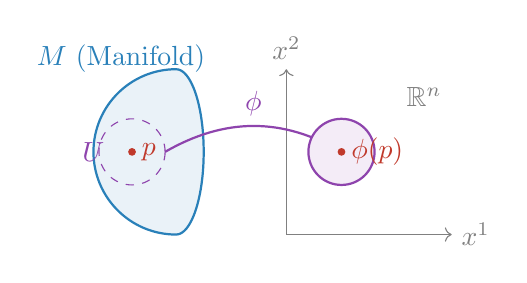
\begin{tikzpicture}[scale=0.7]
        % 流形 M (球面一部分)
        \draw[thick, headerblue, fill=headerblue!10] (0,2) arc (90:270:1.5 and 1.5) arc (-90:90:0.5 and 1.5);
        \node[headerblue] at (-1, 2.2) {$M$ (Manifold)};
        \fill[accentcolor] (-0.8, 0.5) circle (2pt) node[right] {$p$};
        
        % 邻域 U
        \draw[dashed, section2] (-0.8, 0.5) circle (0.6cm);
        \node[section2] at (-1.5, 0.5) {$U$};
        
        % 欧几里得空间 R^n
        \draw[->, gray] (2,-1) -- (5,-1) node[right] {$x^1$};
        \draw[->, gray] (2,-1) -- (2,2) node[above] {$x^2$};
        \node[gray] at (4.5, 1.5) {$\mathbb{R}^n$};
        
        % 映射 phi
        \draw[->, thick, section2, bend left] (-0.2, 0.5) to node[midway, above] {$\phi$} (3, 0.5);
        
        % 像 phi(U)
        \draw[thick, section2, fill=section2!10] (3, 0.5) circle (0.6cm);
        \fill[accentcolor] (3, 0.5) circle (2pt) node[right] {$\phi(p)$};
        
    \end{tikzpicture}
    \end{center}

    \hspace{1em}流形是连接\textbf{局部简单} (像 $\mathbb{R}^n$) 与\textbf{全局复杂} (拓扑结构) 的桥梁。
    \vspace{4pt}
    
    \subt{三大核心视角}
    \begin{itemize}[itemsep=4pt]
        \item \textbf{局部线性化}: 
        切空间 $T_pM$ 是流形在一点处的最佳线性逼近。微积分的所有威力 (导数、积分) 都在这里施展。
        
        \item \textbf{坐标无关性}: 
        真正的物理定律 (如 $F=ma$, 麦克斯韦方程) 不应该依赖于你选择直角坐标还是球坐标。张量分析就是为了书写这种“坐标无关”的真理。
        
        \item \textbf{内蕴几何}: 
        高斯绝妙定理:蚂蚁不需要跳出球面,只需要测量三角形内角和,就能知道自己生活在弯曲的空间里。
    \end{itemize}
    
    \vspace{6pt}
    \centering\textit{\footnotesize 所有的空间都是平的,只要你看得足够近。}
\end{mybox}

\end{multicols*}

\end{document}
